% Messwerte: Alle gemessenen Größen tabellarisch darstellen
% Auswertung: Berechnung geforderter Ergebnisse mit Schritten/Fehlerformeln/Erläuterung/Grafik (Programme)
\section{Auswertung}
\label{sec:auswertung}

\begin{table}
	\label{tab:allgemein}
	\centering
	\caption{Allgemeine Messergebnisse.}
	\input{build/table_allgemein.tex}
\end{table}

\begin{table}
	\label{tab:speziell}
	\centering
	\caption{Spezielle Messergebnisse.}
	\input{build/table_speziell.tex}
\end{table}

\begin{figure}[H]
	\label{fig:plot}
	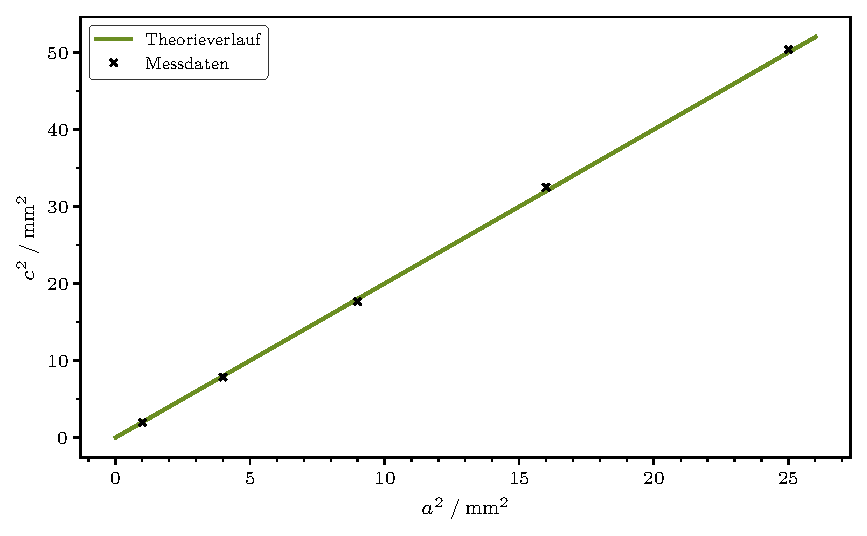
\includegraphics{build/plot.pdf}
	\caption{Messwerte und Theoriegerade.}
\end{figure}

Für $c^2 = ma^2 + n$ liefert \verb+numpy.polyfit+ \cite{numpy}
\begin{align*}
	m = \input{build/m.tex} && n = \input{build/n.tex}
\end{align*}
als Parameter.
